\documentclass[conference]{IEEEtran}
\usepackage[utf8]{inputenc}
\usepackage{graphicx,booktabs,amsmath,amssymb,multirow}
\usepackage{tikz}
\usetikzlibrary{arrows.meta,positioning,fit,backgrounds,calc}
\graphicspath{{figs/}}

\title{Order-Agnostic Autoregressive Diffusion Models on Images and Categorical Tabular Data}
\author{\IEEEauthorblockN{Jorge Barcenilla \quad Santiago Prieto}
\IEEEauthorblockA{Probabilistic Machine Learning, Universidad Carlos III de Madrid\\ Project~I}}

\begin{document}
\maketitle

\begin{abstract}
Order-Agnostic Autoregressive Diffusion Models (OA-ARDMs) unify order-agnostic
autoregressive modelling with absorbing discrete diffusion through a single
masked-prediction objective. We implemented this objective and applied it,
without altering its core, to two distinct modalities: binarized MNIST images
and the fully categorical UCI Mushroom dataset. The tabular case required only
changes to the input parametrization---per-column vocabularies enforced through
masked logits and a dedicated absorbing token---leaving the training and
sampling algorithms identical. For each modality we trained two network
families and measured held-out negative log-likelihood in bits per dimension
(bpd) together with sample fidelity. Convolutional and multilayer-perceptron
backbones reached 0.139 and 0.609 bpd on the MNIST and Mushroom test sets,
produced recognizable digit samples, and reproduced categorical marginals with
mean total-variation distances of 0.17 (MLP) and 0.075 (Transformer). The results show that a single
order-agnostic objective generalizes across heterogeneous data types with only
modality-specific input handling.
\end{abstract}

\section{Introduction}
Deep autoregressive models factorize a joint distribution over $D$ variables
into a product of conditionals $p_\theta(x)=\prod_{d} p_\theta(x_d\mid
x_{<d})$, achieving exact likelihoods but imposing a single fixed generation
order and requiring $D$ sequential network evaluations to sample
\cite{made,pixelcnn}. Order-agnostic autoregressive models relax the fixed
order by treating it as a latent permutation \cite{uria}, while discrete
diffusion models destroy data toward an absorbing state and learn the reverse
process \cite{d3pm}. The Order-Agnostic Autoregressive Diffusion Model
(OA-ARDM) unifies these views: a single shared network is trained, in the
spirit of BERT, to predict an arbitrary masked subset of variables, yielding
flexible order and adaptive parallel sampling \cite{ardm}.

However, the formulation and its public demonstrations are framed almost
exclusively around homogeneous modalities---images and text---in which every
variable shares one vocabulary and a regular spatial or sequential structure.
Whether the same objective transfers cleanly to heterogeneous categorical
tabular data, where each column has a different cardinality and no spatial
adjacency, is not addressed by the original parametrization.

In this paper, we present an implementation of the OA-ARDM and apply its
unmodified training and sampling algorithms to two modalities: binarized MNIST
and the categorical UCI Mushroom dataset. We compare two network families per
modality and evaluate them under a common likelihood metric (bits per
dimension) and under sample-fidelity criteria, isolating the few changes the
tabular setting demands.

\section{Method}
\subsection{Order-agnostic diffusion objective}
Let $x\in\{0,\dots,K-1\}^{D}$ and let $\sigma$ be a permutation of
$\{0,\dots,D-1\}$ drawn uniformly. For a timestep $t\sim\mathcal{U}(1,\dots,D)$
the binary mask $m=(\sigma<t)$ marks the variables already revealed. Masked
variables are replaced by an absorbing value $a$, giving the network input
$i=m\odot x+(1-m)\odot a$. A single shared network $f_\theta$ predicts the
categorical parameters of every masked variable, and training maximizes the
one-term estimator of the likelihood bound
\begin{equation}
\log p(x)\;\ge\;\mathbb{E}_{t\sim\mathcal{U}(1,\dots,D)}\big[\,D\cdot L_t\,\big],
\end{equation}
where $L_t$ is the average log-likelihood over the masked variables at step
$t$ \cite{ardm}. Sampling reverses the process: starting from a fully absorbed
vector, variables are revealed one at a time along $\sigma$, each drawn from
the network's predicted categorical (Fig.~\ref{fig:schema}).

\begin{figure}[t]
\centering
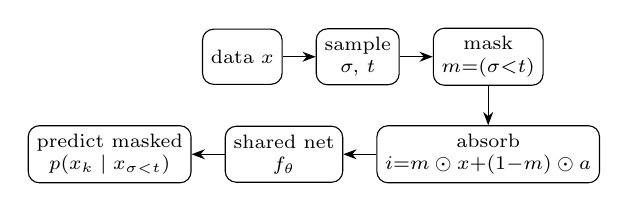
\begin{tikzpicture}[
  box/.style={draw,rounded corners,align=center,inner sep=3pt,font=\scriptsize,minimum height=7mm},
  >=Stealth,node distance=4.2mm]
\node[box] (x) {data $x$};
\node[box,right=of x] (st) {sample\\ $\sigma,\,t$};
\node[box,right=of st] (mask) {mask\\ $m{=}(\sigma{<}t)$};
\node[box,below=5mm of mask] (abs) {absorb\\ $i{=}m\odot x{+}(1{-}m)\odot a$};
\node[box,left=of abs] (net) {shared net\\ $f_\theta$};
\node[box,left=of net] (pred) {predict masked\\ $p(x_k\mid x_{\sigma<t})$};
\draw[->] (x)--(st); \draw[->] (st)--(mask); \draw[->] (mask)--(abs);
\draw[->] (abs)--(net); \draw[->] (net)--(pred);
\end{tikzpicture}
\caption{One training/sampling step of the OA-ARDM. The same objective and
network are reused across both modalities; only the input parametrization
($a$, the vocabulary, and $f_\theta$) is modality-specific.}
\label{fig:schema}
\end{figure}

\subsection{Two instantiations}
The objective above is modality-agnostic. For images, $x$ is a binarized
$28\times28$ digit ($D{=}784$, $K{=}2$); the absorbing value is $0$ and
$f_\theta$ is either a convolutional network with a time embedding
(LeNetWithTime) or a small vision transformer over $7\times7$ patches
(TinyTimeViT). For tabular data, $x$ is a row of $D{=}22$ categorical columns of
differing cardinality (2--12), which breaks the single-vocabulary assumption.
We use one shared vocabulary of size $K{=}\max_j K_j+1$ whose last index is a
dedicated absorbing token (avoiding collision with a valid category), and we
enforce per-column validity by masking the logits of categories absent from a
column to $-\infty$. Each column is embedded as a token (value,
column-identity, and mask embeddings) and processed by either a multilayer
perceptron (MLPWithTime) or a Transformer encoder over the column tokens
(TabTransformer). Training and sampling are otherwise identical to the image
case.

\section{Experimental Setup}
MNIST was binarized at threshold $0.5$ and split into 55{,}000 training,
5{,}000 validation and the standard 10{,}000 test images. The UCI Mushroom
dataset~\cite{mushroom} was encoded
column-wise (missing values as their own category, the constant \texttt{veil-
type} column dropped) with the edible/poisonous label modelled as an additional
column, and split 70/15/15 stratified on the label. All models were trained
with Adam (learning rate $10^{-3}$): 15 epochs for MNIST, 40 for Mushroom.
We report negative log-likelihood as bits per dimension,
$\mathrm{bpd}=\mathrm{NLL}_{\text{nats}}/(D\ln 2)$, estimating the stochastic
objective with $K$ Monte-Carlo repetitions per held-out batch. Sample fidelity
for the tabular models is summarized by the mean per-column total-variation
distance (TVD) between $2{,}000$ generated rows and the test set.

\section{Results}
Table~\ref{tab:results} reports train, validation and test bits per dimension
for all four models, together with the tabular sample-fidelity metric; in every
case train and test values differ by less than $0.01$. Per-label tabular test
bpd for the MLP was 0.629 (edible) and 0.588 (poisonous). Figure~\ref{fig:curves}
shows the optimization trajectories, Figure~\ref{fig:mnist} the unconditional
MNIST samples, and Figure~\ref{fig:marg} the generated versus empirical category
marginals for both tabular models.

\begin{table}[t]
\caption{Held-out negative log-likelihood (bits per dimension) and tabular sample fidelity.}
\label{tab:results}
\centering\footnotesize
\begin{tabular}{@{}llcccc@{}}
\toprule
Data & Model & Train & Val & Test & TVD \\
\midrule
\multirow{2}{*}{MNIST}
 & LeNetWithTime & 0.139 & 0.140 & \textbf{0.139} & --- \\
 & TinyTimeViT   & 0.164 & 0.160 & 0.159 & --- \\
\midrule
\multirow{2}{*}{Mushroom}
 & MLPWithTime    & 0.603 & 0.613 & \textbf{0.609} & 0.17 \\
 & TabTransformer & 0.677 & 0.683 & 0.667 & \textbf{0.075} \\
\bottomrule
\end{tabular}
\end{table}

\begin{figure}[t]
\centering

\includegraphics[width=\columnwidth]{curves.pdf}
\caption{Training (solid) and validation (dashed) bits per dimension. Left:
MNIST. Right: Mushroom.}
\label{fig:curves}
\end{figure}

\begin{figure}[t]
\centering
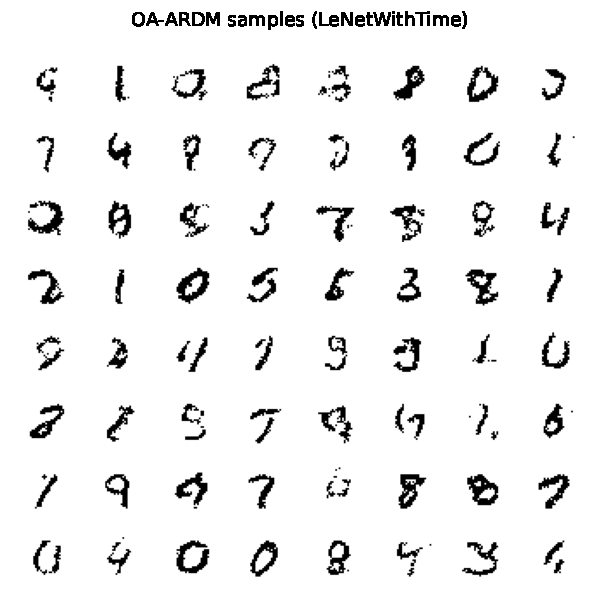
\includegraphics[width=0.78\columnwidth]{mnist_samples.pdf}
\caption{Unconditional samples generated by the order-agnostic sampler
(LeNetWithTime, binarized MNIST).}
\label{fig:mnist}
\end{figure}

\section{Discussion}
The objective was met: an unaltered order-agnostic diffusion core produced
calibrated likelihoods and plausible samples in both an image and a categorical
tabular setting, with the tabular adaptation confined to the input
parametrization. The MNIST test bpd of 0.139 is consistent with reported
order-agnostic results on binarized MNIST \cite{ardm}, supporting the
correctness of the implementation. In both modalities the smaller backbone
(convolutional or perceptron) attained lower likelihood than its transformer
counterpart, which we attribute to the modest model size and training budget
relative to the transformer's capacity. Likelihood and sample fidelity did not
coincide on the tabular data: the MLP achieved the best bpd yet the
TabTransformer reproduced categorical marginals more faithfully
(Fig.~\ref{fig:marg}), a known decoupling between log-likelihood and perceptual
or distributional sample quality.

These findings are bounded by the small networks, the single training seed, and
a sample-fidelity metric that captures only first-order (marginal) structure;
higher-order dependencies between columns were not quantified. Even within these
bounds, the central observation holds across two unrelated datasets: a single
order-agnostic diffusion objective transfers between images and heterogeneous
categorical tables, requiring only a per-column vocabulary and a dedicated
absorbing token rather than any change to training or sampling.

\section{Conclusion}
We implemented an Order-Agnostic Autoregressive Diffusion Model and showed that
its training and sampling algorithms apply unchanged to two distinct
modalities, binarized images and fully categorical tabular data, once the input
parametrization accounts for per-column vocabularies through masked logits and a
dedicated absorbing token. Across both datasets the model produced competitive
held-out likelihoods and faithful samples, demonstrating that a single
order-agnostic objective is a genuinely modality-portable foundation for
discrete generative modelling.

\onecolumn
\appendices
\section{Software Architecture}
The implementation isolates a shared algorithmic core from modality-specific
front-ends (Fig.~\ref{fig:arch}). Two parallel branches---image and
tabular---each provide a data loader, an input-processing module that builds the
masked, time-conditioned features, and a backbone network. Both branches feed
the same two algorithms: the training objective (Algorithm~2) and the
order-agnostic sampler (Algorithm~1). The tabular branch adds a precomputed
per-column validity mask used to project logits onto the categories that each
column admits. The pipelines are reproducible end-to-end
(\texttt{main\_mnist.py}, \texttt{main\_tabular.py}) and the tabular core is
covered by unit tests for masking, the absorbing token, loss back-propagation
and sampler validity.

\begin{figure}[h]
\centering
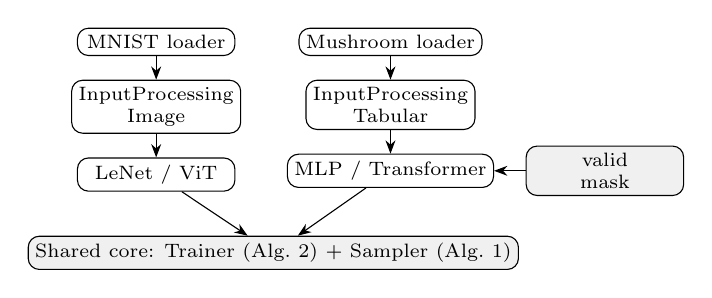
\begin{tikzpicture}[
  b/.style={draw,rounded corners,align=center,font=\scriptsize,inner sep=2.5pt,minimum width=20mm},
  >=Stealth,node distance=3mm]
\node[b] (im) {MNIST loader};
\node[b,right=8mm of im] (tb) {Mushroom loader};
\node[b,below=of im] (ipi) {InputProcessing\\Image};
\node[b,below=of tb] (ipt) {InputProcessing\\Tabular};
\node[b,below=of ipi] (ni) {LeNet / ViT};
\node[b,below=of ipt] (nt) {MLP / Transformer};
\node[b,below=8mm of $(ni)!0.5!(nt)$,fill=black!6,minimum width=46mm] (core)
  {Shared core: Trainer (Alg.~2) + Sampler (Alg.~1)};
\draw[->](im)--(ipi);\draw[->](tb)--(ipt);
\draw[->](ipi)--(ni);\draw[->](ipt)--(nt);
\draw[->](ni)--(core);\draw[->](nt)--(core);
\node[b,right=4mm of nt,fill=black!6] (vm) {valid\\mask};
\draw[->](vm)--(nt);
\end{tikzpicture}
\caption{Module layout: parallel image and tabular front-ends share one
training/sampling core.}
\label{fig:arch}
\end{figure}

\begin{figure}[h]
\centering

\includegraphics[width=0.7\textwidth]{tabular_marginals.pdf}
\caption{Empirical (blue) versus generated (orange) category marginals on the
Mushroom test set for three representative columns. Top: MLPWithTime. Bottom:
TabTransformer.}
\label{fig:marg}
\end{figure}

\begin{thebibliography}{1}
\footnotesize
\bibitem{ardm} E. Hoogeboom \emph{et al.}, ``Autoregressive Diffusion Models,''
\emph{ICLR}, 2022.
\bibitem{made} M. Germain \emph{et al.}, ``MADE: Masked Autoencoder for
Distribution Estimation,'' \emph{ICML}, 2015.
\bibitem{uria} B. Uria \emph{et al.}, ``A Deep and Tractable Density
Estimator,'' \emph{ICML}, 2014.
\bibitem{d3pm} J. Austin \emph{et al.}, ``Structured Denoising Diffusion Models
in Discrete State-Spaces,'' \emph{NeurIPS}, 2021.
\bibitem{pixelcnn} A. van den Oord \emph{et al.}, ``Pixel Recurrent Neural
Networks,'' \emph{ICML}, 2016.
\bibitem{mushroom} J. Schlimmer, ``Mushroom Data Set,'' UCI Machine Learning
Repository, 1987.
\end{thebibliography}

\end{document}
